\chapter{Motor Imagery: the hunt for a greek letter}
\label{chapter:five}
\epigraph{...utilizing the brain signals in man-computer dialogue.}{Vidal}

\section{Introduction}

Motor Imagery is an EEG or ECoG based BCI paradigm originated on changes of SMR, sensorimotor rhythms, that are altered when a person engages in motor behavior, but it can also be elicited when a person imagines to perform any movement. Particularly, the Rolandic wicket rhythm, the $\mu$ rhythm, is of the same frequency (e.g. 8-12 Hz) of visual occipital alpha waves, but from a spatially different location (posterior frontal and anterior parietal areas)\cite{WolpawJonathanR2012}.   Although SMR patterns presents a high inter- and intra-subjects variability regarding the signal features required to identify them, an Event Related Desynchronization/Synchronization of $\mu$ rhythm is in general consistent across subjects, regardless of the specificity of the imagined movement (i.e. what is being imagined to move).

\section{Materials and Methods}

In order to verify if this ERD/ERS could be detected by the method presented in this Thesis, i.e. by automatically extracting the information from the signal plots, a BCI Simulation is performed against the public Motor Imagery Dataset 002-2014, published by BNCI-Horizon 2020 website and initiative~\cite{Steyrl2015}.  This dataset is composed of channels C3, Cz and C4.  Four surrounding channels are also provided on each of these electrodes conforming a spatial Laplacian arrangement. The protocol consisted of 8 runs for 14 participants, aged between 20 and 30 years, five females, with a sampling frequency of $\gls{Fs} = 512$. Nine out of these 14 participant reported never been exposed to a BCI device.  One session per participant is recorded on a single day and one session consisted of eight consecutive runs with short pauses between them.  The first 5 runs are used for training without feedback, and the remaining 3 runs are used to test the results.  The original online experiment was performed with 20 trials on each run, 10 corresponding to imagining moving the right hand and the other 10 to feet movement.  Figure~\ref{fig:midatasetdiagram} schematize the protocol and the structure of this published dataset.  This BCI simulation experiment is divided in two.  In the first simulation, baseline signals, corresponding to the 1st second of each trial are compared against right hand motor imagery, which is 4.5 seconds ahead of the beginning of each trial. Signal segments of 1-second length are processed for 10 trials for each of 5 runs and their descriptors are extracted for both classes.  The second BCI simulation is similar but only extracting trials corresponding to feet movement imagery.



\begin{story}[BCI Simulation or Cross Validation?]
The task of decoding information from brain signals inherits practices from Machine Learning (ML).  Cross-validation is used in ML to reduce overfitting bias and to increase the independence on the dataset that is used as calibration (see Section~\ref{Calibration}).  However, the brain data used in BCI is extracted from a person who is performing a task and whose signals are changing while trying to adapt to this operation.  Hence, mixing the dataset, shuffling the sessions and trials is at least a challenging assumption.  BCI Simulation, on the other hand, is not very well defined in BCI research, but their practice, without naming it, has been the regular approach for BCI Competitions. It consists in reproducing the operational sequence that was utilized to generate the dataset. Hence, the experiment is replicated offline using the training information to train or calibrate a classifier, and to classify the testing signals as if they were generated at that same moment.

Regardless of any definition, the online validation with feedback of any BCI system is the unquestioned gold standard of the discipline~\cite{WolpawJonathanR2012}.
\end{story}


\begin{figure}[]
\centering
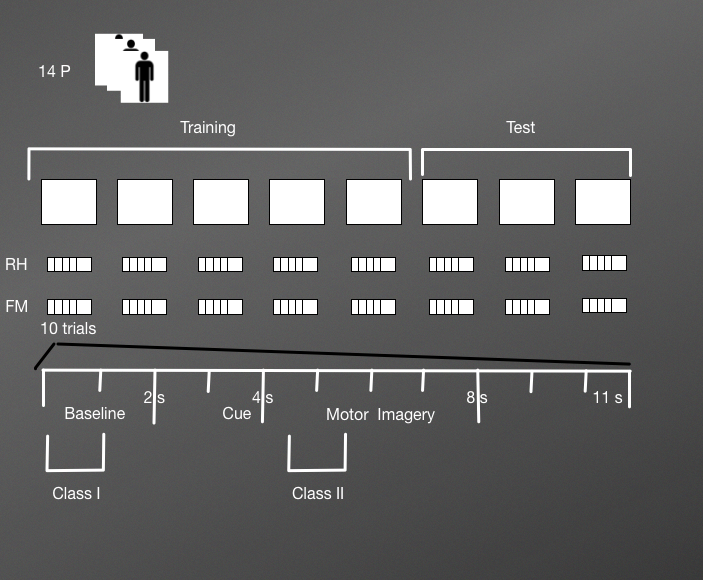
\includegraphics[scale=0.6]{images/DatasetIIIDiagram2.png}
\caption[Motor Imagery Experimental Protocol]{Fourteen voluntary participants performed 5 sessions of training and 3 sessions of testing.  On each session each subject had 10 trials to perform Right Hand Motor Imagery (RH) and 10 trials for Feet Movement (FM).  At the same time, each trial has a 2-seconds baseline and a 4-seconds section to perform the imagery task.  For each BCI Simulation, class 1 is defined from the EEG segments obtained from the baseline section, while class 2 is based on extracting segments from the imagery section of the EEG signal.}
\label{fig:midatasetdiagram}
\end{figure}


\section{Results}

Binary classification accuracies are calculated based on the output of the BCI simulation on the remaining 3 runs for each participant, in a single-trial approach: for each sampled segment of 1-second length, classification based on the classification algorithm described in \ref{nbnn} is applied and a match or mismatch is obtained.  Results are shown in Figure~\ref{fig:miresults} where for right-hand detection \textit{RH}, average accuracies of around $70\%$ are obtained for the channel C3, the best-performing channel $\gls{bpc}$, coincidentally with the contralateral structure of the imagined movement.  On the other hand, the binary classification accuracy for feet imagery detection \textit{FM}, achieves in all the channels accuracies of just above chance level.

   
\begin{figure}[h!]
\centering
\subfigure[]
{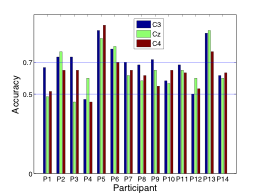
\includegraphics[width=7cm, height=5cm]{images/MIinformedonpaper1.png}}
\subfigure[]
{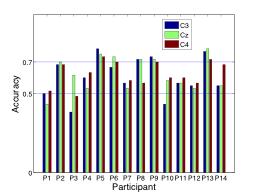
\includegraphics[width=7cm, height=5cm]{images/MIinformedonpaper2.png}}
\caption[Motor Imagery Accuracy]{Classification Accuracy for discriminating segments of 1s ($\gls{N} = 512$) of EEG for Motor Imagery detection BCI simulation. (a) Accuracy values for channels C3, Cz and C4 for the 14 participants of the described MI dataset discriminating between baseline and right-hand imagery. (b) The same procedure for feet imagery. Accuracy levels averaged to $70\%$ are obtained only for right-hand movement on the contralateral channel C3. The horizontal $\gls{St}$ and vertical $\gls{Sv}$ patch scale are adjusted to $6$, while the amplitude scale factor $\gls{gamma}$ and time scale factor $\gls{gammat}$ are set equal to $2$.  This gives an span $\gls{lambda} = 0.12$  $\si{s}$ and maximum peak-to-peak amplitude $\gls{DeltamuV}$ of $64 \; \mu V$.  }
\label{fig:miresults}
\end{figure}
   
\section{Conclusion}

Offline BCI Simulation of single trial asynchronous triggering for right hand MI based on signal plots is implemented with a level of success of $70\%$ for 7 out of 14 Participants. Single trial asynchronous triggering of BCI can be implemented with this paradigm, particularly for right-hand motor imagery. The name $\mu$ rhythm was precisely coined because the shape of the waves have some resemblance to the greek letter~\cite{Cole2017}.   Additionally, in line with previous chapter results, though the differentiation information is contained in the frequency domain, the method based on the Histogram of Gradient Orientation detected differences in the shape of the signals.  Coincidentally with results obtained from Alpha Waves, there is information that is mapped in the structure of the waveform, at least for frequencies on the 10 Hz range, which characterize both types of waves.

% Parameters
% Poner una figura donde más o menos se vean las señales.


